\documentclass{article}
\usepackage[utf8]{inputenc}

\title{100 Ideias}
\author{Andre Carvalho\\  Andre Fonseca\\ Bruno Cabral  \\ Tiago Castanheira\\ }
\date{April}

\usepackage{natbib}
\usepackage{graphicx}

\begin{document}
\keywords{Helping\\ Caring \\ Integration}
\maketitle
\begin{abstract}
    Ajudar os refugiados garantindo que existem vários apoios aos refugiados, ajudando a fazer as suas decisões sobre que cidades escolher , usando para isso um website.\\
    
    Nos observamos que  muitas destas pessoas não conhecem as culturas nas quais querem integram e por esta razão decidimos facilitar a integração na sociedade.\\
    
    \\
    
    Nos esperamos que a nossa contribuição ajude os indivíduos a perceber melhor e a facilitar a sua integração na comunidade \\
    
    
\end{abstract}
\keywordlist

\section{Introduction}

%% The ``\copyrightspace'' command must be the first command after the
%% start of the first section of the body of your paper. It ensures the
%% copyright space is left at the bottom of the first column on the first
%% page of your paper.

%% \copyrightspace

Your project introduction here. Maximum 4 paragraphs. You can
follow this structure

\begin{itemize}
    \item paragraph 1: describe what is the problem and why it is
    interesting.
    \item paragraph 2: state the goal of the project.
    \item paragraph 3: describe (briefly) the approach you will
    follow and the possible results you will generate.
    \item paragraph 4: outline of the article (optional). If the
    article it is too long it is recommended to have this
    paragraph.


\end{itemize}

\section{}



\begin{figure}[h!]
\centering
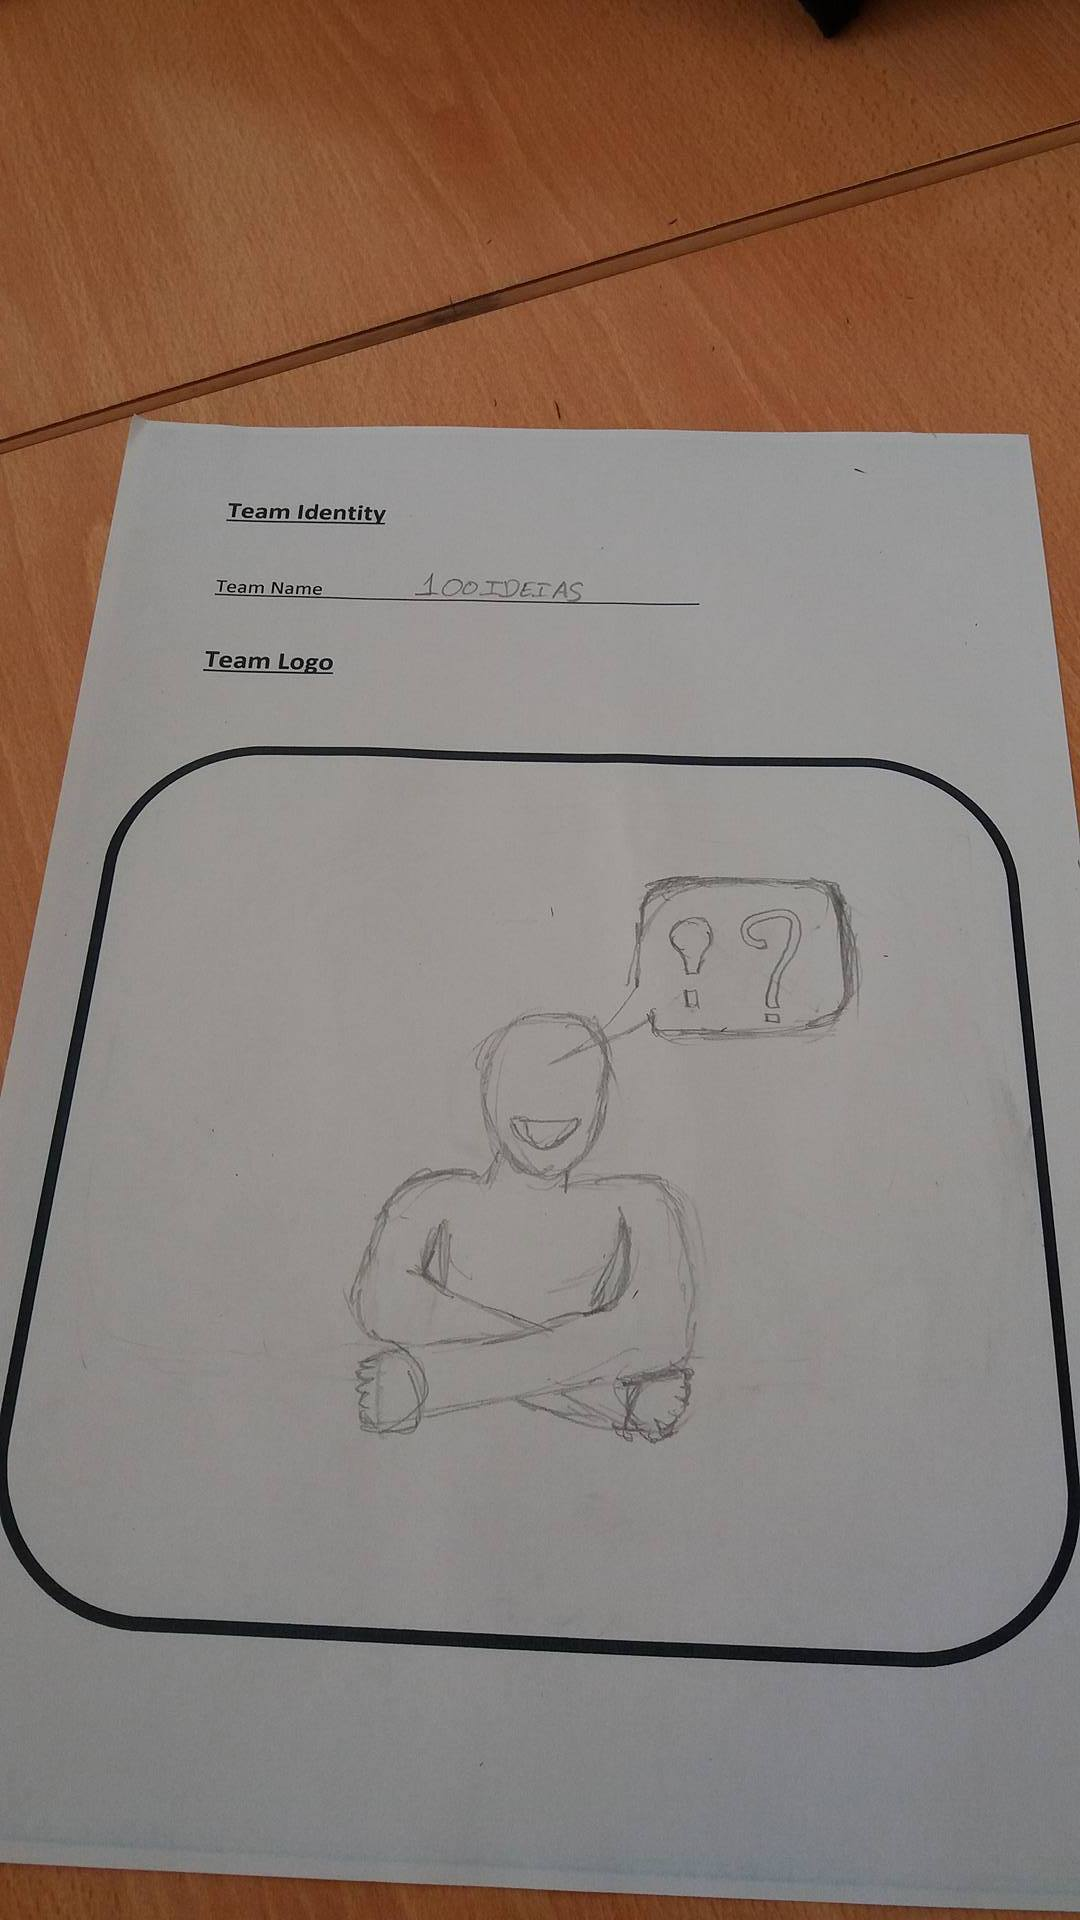
\includegraphics[scale=1.7]{logo.jpg}
\caption{The Universe}
\label{fig:univerise}
\end{figure}

\section{Conclusion}
``I always thought something was fundamentally wrong with the universe'' \citep{adams1995hitchhiker}

\bibliographystyle{plain}
\bibliography{references}
\end{document}
